\documentclass[12pt]{article}
\usepackage[utf8]{inputenc}
\usepackage[T5]{fontenc}
\usepackage{graphicx,a4wide,framed}

\newcommand{\source}[1]{\begin{flushright}\emph{[#1]}\end{flushright}}

\title{PC1 : Diviser pour régner et algorithmes gloutons}
\author{École Centrale-Supélec --- Christoph Dürr, Nguyễn Kim Thắng}
\date{Algorthmique Avancée, 2018}

%\newcommand{\MakeScribeTop}{
%\noindent
%\begin{center}
%  \framebox{
%    \vbox{
%      \headerwidth=\textwidth
%      \advance\headerwidth by -0.22in
%      \hbox to \headerwidth {{\bf Graphes \& Algorithmes \hfill Dept Informatique, Univ Evry} }
%      \vspace{4mm}
%      \hbox to \headerwidth {{\Large \bf \hfill TD \HomNum: \LecTitle \hfill}}
%      \vspace{2mm}
%      \hbox to \headerwidth {{\it \LecStr \hfill \LecDate}}
%      \hbox to \headerwidth {{\it \TdStr \hfill }}
%      }
%    }
%\end{center}
%\vspace*{4mm}}


\begin{document}
    \maketitle

    \section{Cartes bancaires}



    Vous travaillez pour une banque dans le service des répressions des fraudes.  On vous donne $n$ cartes bancaires qui sont suspectés d'être frauduleuses. Chaque carte bancaire comporte une bande magnétique avec des données crypté correspondant à un compte unique. Plusieurs cartes peuvent être associées à un même compte, et dans ce cas on dit qu'elles sont \emph{équivalentes}.
    Il n'est pas aisé de lire les numéros de compte sur les cartes directement, cependant
    vous disposez d'une technologie qui permet de tester si deux cartes données sont équivalentes.
    La question est de déterminer si parmi les $n$ cartes données, il y a un ensemble d'au moins $n/2$ cartes mutuellement équivalentes.

    Montrez que cette tâche est réalisable avec seulement $O(n \log n)$ utilisations du testeur d'équivalence.

\source{Algorithms Design, Chapitre 5, Exercice 3}

    \section{Placement d'antennes}


\begin{figure}[h]
\centerline{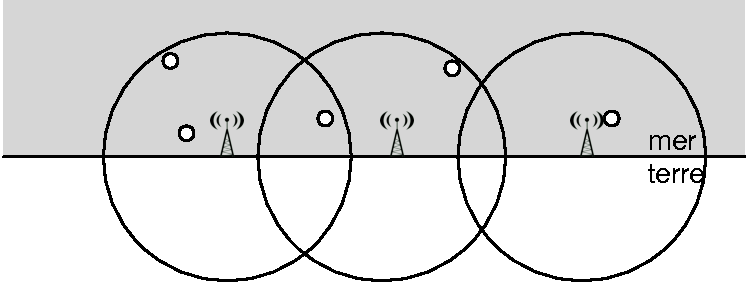
\includegraphics[width=8cm]{radar-disc}}
\caption{Exemple (non-optimal) de placement d'antennes}
\end{figure}

Soit une plage toute droite et des îles, aussi petites que des points.
Toutes les îles sont à distance au plus $r$ de la plage.
Nous voulons placer les antennes le long de la plage pour couvrir toutes les îles.
Chaque antenne peut couvrir les îles dans un rayon $r$.
Donnez un algorithme qui place un nombre minimum d'antennes pour couvrir toutes les îles.  

\source{Programmation efficace, section 5.3}


\section{Gestion de cache}

Le cache est une mémoire intercalée entre la mémoire et le processeur.
La mémoire principale est divisée en $n$ blocs de même taille.  Ces blocs sont appelés \emph{pages}.
Les accès au cache sont plus rapides qu'à la mémoire principale,
mais pour des raisons de coût il a une capacité plus petite.  Le cache peut contenir $k$ pages, avec $k \ll n$.
Les accès mémoire du processeur se traduisent en requêtes à des pages. Si la page en question est dans le cache, la requête peut être servi immédiatement. Dans le cas échéant on parle de \emph{faute de cache}. Le mécanisme de gestion de cache doit alors choisir une page actuellement dans le cache pour l'échanger avec la page demandée.  Cette opération est lente.  Le but est de minimiser le nombre de fautes de cache, en prenant des bonnes décisions sur les échanges de pages.

Initialement le cache est vide, et les $k$ première fautes de caches provoquent un chargement de la nouvelle page plutôt qu'un remplacement.  Par conséquence on ne tient pas compte de ces $k$ premières fautes de cache.


\begin{figure}[hp]
\begin{center}
\begin{tabular}{l||*{14}c}
requêtes &
2 & 3 & 4 & 2 & \underline{1} & 3 & \underline{7} & \underline{5} & 4 & 1 & \underline{3} & \underline{2} & 4 & 1
\\ \hline
cache
& 2 & 2 & 2 & & 1 & & 1 & 1 & & & 1 & 1 \\
& - & 3 & 3 & & 3 & & 7 & 5 & & & 3 & 2 \\
& - & - & 4 & & 4 & & 4 & 4 & & & 4 & 4 \\
\end{tabular}
\end{center}
\caption{Exemple de gestion du cache pour un capacité de $k=3$. Les fautes de cache sont soulignées.}
\end{figure}

On se place dans une situation simplifiée où toutes les requêtes sont connues en avance.
Considérez l'algorithme de gestion de cache suivant (proposé par László Bélády dans les années 60).

\begin{framed}
    \textsc{Furthest-in-Future} (FF): En cas de faute de cache, échanger la page demandée avec une page du cache dont la prochaine requête est la plus loin dans le futur.
\end{framed}

On va prouver l'optimalité de l'algorithme FF par induction.
%Fixez une instance arbitraire et considérez un algorithme A arbitraire.
Montrez que si le comportement d'un algorithme A est identique avec celui de FF sur les $i$ premières requêtes, alors il existe un algorithme B qui est identique avec FF sur les $(i+1)$ premières requêtes et qui ne provoque pas plus de fautes de cache que l'algorithme A.

\end{document}